\documentclass{article}

\usepackage[table,xcdraw]{xcolor}
\usepackage{fancyhdr}
\usepackage{extramarks}
\usepackage{amsmath}
\usepackage{amsthm}
\usepackage{amsfonts}
\usepackage{tikz}
\usepackage[plain]{algorithm}
\usepackage{algpseudocode}
\usepackage{enumerate}

\usepackage{listings}
\usepackage{forest}
\usepackage[shortlabels]{enumitem}

\usepackage{pgfplots}
\usepackage{wrapfig}


\setlist[enumerate, 1]{1\textsuperscript{o}}
\lstset { %
    language=C++,
        backgroundcolor=\color{black!5}, % set backgroundcolor
            basicstyle=\footnotesize,% basic font setting
}

%\usetikzlibrary{automata,positioning}
\usetikzlibrary{positioning,shapes,shadows,arrows,automata}

%
% Basic Document Settings
%

\topmargin=-0.45in
\evensidemargin=0in
\oddsidemargin=0in
\textwidth=6.5in
\textheight=9.0in
\headsep=0.25in

\linespread{1.1}

\pagestyle{fancy}
\lhead{\hmwkAuthorName}
\rhead{ (\hmwkClassInstructor\ \hmwkClassTime): \hmwkTitle}
\lfoot{\lastxmark}
\cfoot{\thepage}

\renewcommand\headrulewidth{0.4pt}
\renewcommand\footrulewidth{0.4pt}

\setlength\parindent{0pt}

%
% Create Problem Sections
%

\newcommand{\enterProblemHeader}[1]{
    \nobreak\extramarks{  }{Problem \arabic{#1} continued on next page\ldots}\nobreak{  }
    \nobreak\extramarks{Problem \arabic{#1} (continued)}{Problem \arabic{#1} continued on next page\ldots}\nobreak{  }
}

\newcommand{\exitProblemHeader}[1]{
    \nobreak\extramarks{Problem \arabic{#1} (continued)}{Problem \arabic{#1} continued on next page\ldots}\nobreak{  }
    \stepcounter{#1}
    \nobreak\extramarks{Problem \arabic{#1}}{  }\nobreak{  }
}

\setcounter{secnumdepth}{0}
\newcounter{partCounter}


\newcommand{\hmwkTitle}{Assignment \#4}
\newcommand{\hmwkDueDate}{June 1st, 2016}
\newcommand{\hmwkClass}{CS515 Parallel Programming}
\newcommand{\hmwkClassTime}{Spring 2016}
\newcommand{\hmwkClassInstructor}{Jingke Li}
\newcommand{\hmwkAuthorName}{Konstantin Macarenco}


\title{
    \vspace{2in}
    \textmd{\textbf{\hmwkClass:\ \hmwkTitle}}\\
        \normalsize\vspace{0.1in}\small{Due\ on\ \hmwkDueDate\ at 11:59pm}\\
        \vspace{0.1in}\large{\textit{\hmwkClassInstructor\ \hmwkClassTime}}
    \vspace{3in}
}

\author{\textbf{\hmwkAuthorName}}
\date{  }

\renewcommand{\part}[1]{\textbf{\large Part \Alph{partCounter}}\stepcounter{partCounter}\\}

%
% Various Helper Commands
%

% Useful for algorithms
\newcommand{\alg}[1]{\textsc{\bfseries \footnotesize #1}}

% For derivatives
\newcommand{\deriv}[1]{\frac{\mathrm{d}}{\mathrm{d}x} (#1)}

% For partial derivatives
\newcommand{\pderiv}[2]{\frac{\partial}{\partial #1} (#2)}

% Integral dx
\newcommand{\dx}{\mathrm{d}x}

% Alias for the Solution section header
\newcommand{\solution}{\textbf{\large Solution}}

% Probability commands: Expectation, Variance, Covariance, Bias
\newcommand{\E}{\mathrm{E}}
\newcommand{\Var}{\mathrm{Var}}
\newcommand{\Cov}{\mathrm{Cov}}
\newcommand{\Bias}{\mathrm{Bias}}

\begin{document}
\maketitle

\pagebreak

\section{Implementation details}

Implementation of ``C'' version was straight forward and didn't cause any problems,
converting Jacobi to Gauss was simple - reuse the same matrix when preforming the
computation.
\begin{lstlisting}
for (i = 1; i < n-1; i++) {
    for (j = 1; j < n-1; j++) { ...
        old = x[i][j]
        x[i][j] = ...
\end{lstlisting}

Conversion from Gauss-Seidel normal order to Red-Black, order is implemented by using 4
loops:
\begin{lstlisting}
for (i = 1; i < n-1; i = i + 2) { // Red - odd column odd row (row + column \% 2 := 0)
    for (j = 1; j < n-1; j = j + 2) { ...

for (i = 2; i < n-1; i = i + 2) { // Red  - even column even row (row + column \% 2 := 0)
    for (j = 2; j < n-1; j = j + 2) { ...

for (i = 1; i < n-1; i = i + 2) { // Black - odd column even row (row + column \% 2 := 1)
    for (j = 2; j < n-1; j = j + 2) { ...

for (i = 2; i < n-1; i = i + 2) { // Black - even column odd row (row + column \% 2 := 1)
    for (j = 1; j < n-1; j = j + 2) { ...
\end{lstlisting}

In Chapel Implementation looks quite similar, except for language specifics:
\begin{lstlisting}
forall ij in innerDomain do { const innerDomain = BD[{1..n-2,1..n-2}];

\end{lstlisting}
\begin{lstlisting}
forall ij in BDr1 do { ... // const BDr1 = BD[1..n-2 by 2, 1..n-2 by 2];
forall ij in BDr2 do { ... // const BDr2 = BD[2..n-2 by 2, 2..n-2 by 2];
forall ij in BDb1 do { ... // const BDb1 = BD[1..n-2 by 2, 2..n-2 by 2];
forall ij in BDb2 do { ... // const BDb2 = BD[2..n-2 by 2, 1..n-2 by 2];
\end{lstlisting}

It can be done in two loops, however this way's advantage - there is no need to calculate
correct row offset. \\

\section{Performance}

Chapel aims to make writing of parallel applications easy, and provides many built in
mechanisms for this purpose. I enjoyed developing in Chapel, however the main problem with
this language is performance (not sure if this is due to language problems or to my
particular implementation of the Laplace algorithms). Sequential ``C'' is up to x9 times
faster than similar shared memory algorithm in Chapel. \\

Distributed version written in Chapel required very little modifications to the original
code - only correct mapping to the locales, however it was even slower than shared memory,
with number locales doubled performance is slowed down by x2.
Such a significant slowdown can be explained by high cost of communication between border
locales, or by poor Implementation/Compilation of PGAS features.

In distributed version I verified locales affinity by creating functions with exactly the
same semantics as Jacobi - Gauss methods, except instead of performing computation it records
locale ID", and by adding print statement that outputs number of current locale and current matrix
element locale. Printout can be enabled by setting verbose flag to $>0$.\\

\pagebreak

Convergence of all implementations is almost identical with insignificant deviations $\pm
\%1- 2$.
Gauss-Seidel convergence rate (both versions), is around \%40 better than Jacobi, this was
expected since values propagate faster, when update happens ``in place''. Gauss-Seidel and Red-Black
have about the same convergence rate, with Red-Black faster by some constant. The biggest downside
of Red-Black, - need of at least two scans of the array, one for Red Cells and another for Black, 
which requires additional synchronization, however there is no potential concurrent writes as in
Normal order.
Shared memory version of Gauss-Seidel is usually faster, by a constant despite having a slower
convergence rate. \\

% Convergence
% Jacobi,Gauss-Seidel,Red-Black
% 43  , 27  , 26  , 8
% 131 , 86  , 82  , 16
% 285 , 215 , 208 , 32
% 360 , 357 , 347 , 64 % 360 , 374 , 361 , 128
% 360 , 374 , 361 , 256

\noindent\makebox[\linewidth]{\rule{\textwidth}{0.4pt}}

With rough convergence tolerance, changes quickly propagate through the matrix, hence larger
dimension have the same number of convergence steps, and vice versa:
\\

\begin{minipage}{0.52\textwidth}
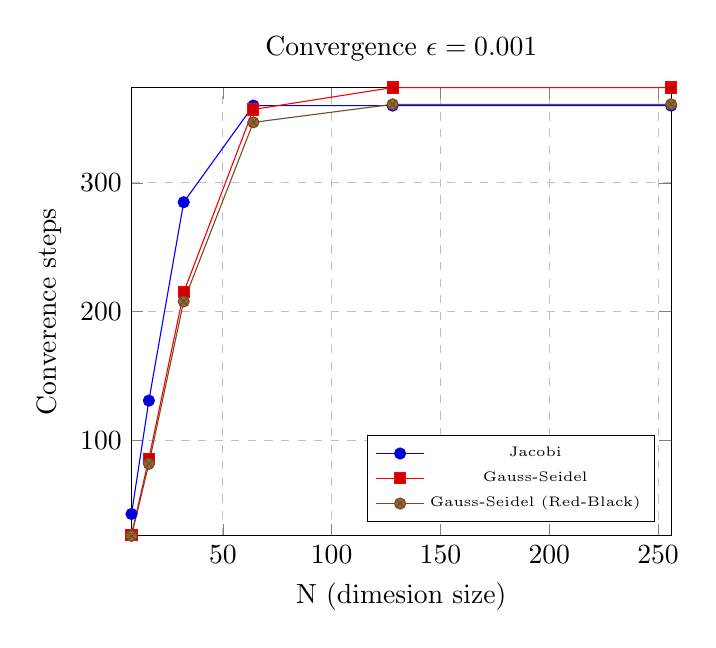
\begin{tikzpicture}
\begin{axis}[
title={Convergence $\epsilon = 0.001$},
xlabel={N (dimesion size)},
ylabel={Converence steps},
ymajorgrids=true,
xmajorgrids=true,
grid style=dashed,
enlargelimits=false,
scaled y ticks=false,
legend style={legend pos=south east, font=\fontsize{4}{5}\selectfont},
]
\addplot coordinates {
(8       , 43    )
(16      , 131   )
(32      , 285   )
(64      , 360   )
(128     , 360   )
(256     , 360   )
}; \addlegendentry{Jacobi}

\addplot coordinates {
(8       , 27   )
(16      , 86   )
(32      , 215  )
(64      , 357  )
(128     , 374    )
(256     , 374    )
}; \addlegendentry{Gauss-Seidel}

\addplot coordinates {
(8       , 26   )
(16      , 82   )
(32      , 208  )
(64      , 347  )
(128     , 361  )
(256     , 361  )
}; \addlegendentry{Gauss-Seidel (Red-Black)}

\end{axis}
\end{tikzpicture}
\end{minipage}%
\begin{minipage}{0.52\textwidth}
%Jacobi,Gauss-Seidel,Red-Black
%87    , 49    , 48    , 8
%339   , 190   , 186   , 16
%1173  , 662   , 655   , 32
%3709  , 2150  , 2134  , 64
%10495 , 6412  , 6381  , 128
%24121 , 16610 , 16550 , 256


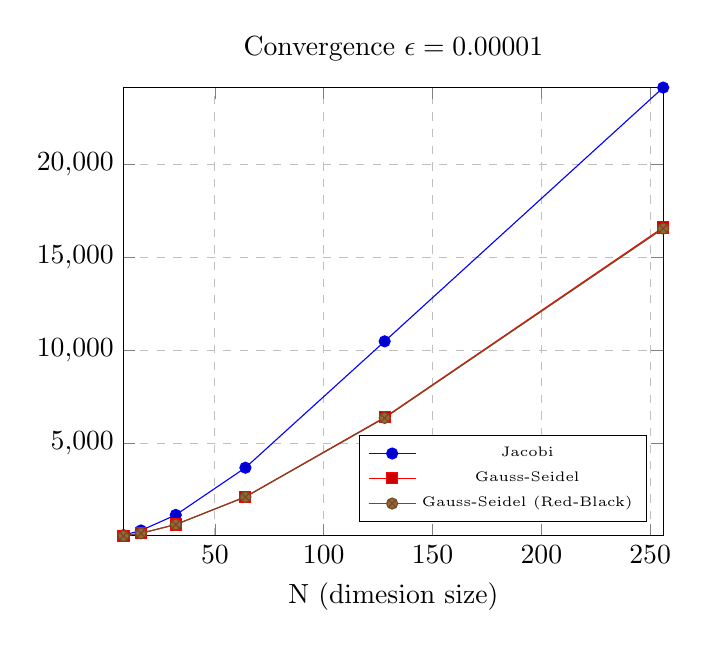
\begin{tikzpicture}
\begin{axis}[
title={Convergence $\epsilon = 0.00001$},
xlabel={N (dimesion size)},
ymajorgrids=true,
xmajorgrids=true,
grid style=dashed,
enlargelimits=false,
scaled y ticks=false,
legend style={legend pos=south east, font=\fontsize{4}{5}\selectfont},
]

\addplot coordinates {
(8       , 87      )
(16      , 339     )
(32      , 1173    )
(64      , 3709    )
(128     , 10495   )
(256     , 24121   )
}; \addlegendentry{Jacobi}

\addplot coordinates {
(8       , 49    )
(16      , 190   )
(32      , 662   )
(64      , 2150  )
(128     , 6412    )
(256     , 16610   )
}; \addlegendentry{Gauss-Seidel}

\addplot coordinates {
(8       , 48      )
(16      , 186     )
(32      , 655     )
(64      , 2134    )
(128     , 6381    )
(256     , 16550   )
}; \addlegendentry{Gauss-Seidel (Red-Black)}
\end{axis}
\end{tikzpicture}
\end{minipage}%

\vspace{0.6cm}
\noindent\makebox[\linewidth]{\rule{\textwidth}{0.4pt}}
Performance of shared memory vs sequential implementation (Chapel):

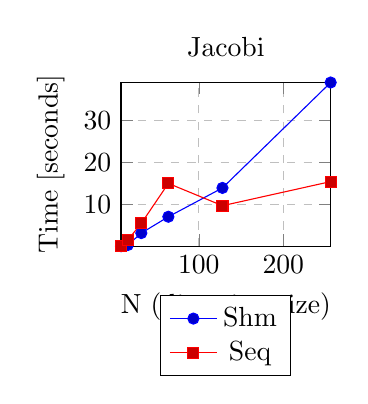
\begin{tikzpicture}
\begin{axis}[
title={Jacobi},
xlabel={N (dimesion size)},
ylabel={Time [seconds]},
ymajorgrids=true,
xmajorgrids=true,
grid style=dashed,
enlargelimits=false,
scaled y ticks=false,
width=0.35\textwidth, 
legend style={at={(0.5,-0.30)},anchor=north,legend columns=1},
%legend style={legend pos=south east, font=\fontsize{4}{5}\selectfont},
]

\addplot coordinates {
(8       , 0.057792    )
(16      , 0.326193    )
(32      , 3.18076     )
(64      , 7.08417     )
(128     , 13.9652     )
(256     , 39.1292     )
}; \addlegendentry{Shm}

\addplot coordinates {
(8       , 0.169748   )
(16      , 1.53658    )
(32      , 5.50225    )
(64      , 15.0425    )
(128     , 9.71945      )
(256     , 15.4735      )
}; \addlegendentry{Seq}

\end{axis}
\end{tikzpicture}
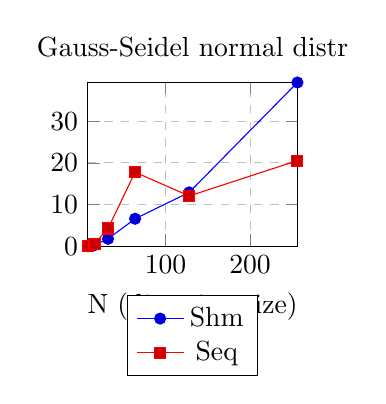
\begin{tikzpicture}
\begin{axis}[
title={Gauss-Seidel normal distr},
xlabel={N (dimesion size)},
ymajorgrids=true,
xmajorgrids=true,
grid style=dashed,
enlargelimits=false,
scaled y ticks=false,
width=0.35\textwidth, 
legend style={at={(0.5,-0.30)},anchor=north,legend columns=1},
%legend style={legend pos=south east, font=\fontsize{4}{5}\selectfont},
]

\addplot coordinates {
(8       , 0.01843    )
(16      , 0.269015   )
(32      , 1.78843    )
(64      , 6.59587    )
(128     , 12.9231    )
(256     , 39.276     )
}; \addlegendentry{Shm}

\addplot coordinates {
(8       , 0.096871  )
(16      , 0.572665  )
(32      , 4.27667   )
(64      , 17.764    )
(128     , 12.0583   )
(256     , 20.5423   )
}; \addlegendentry{Seq}
\end{axis}
\end{tikzpicture}
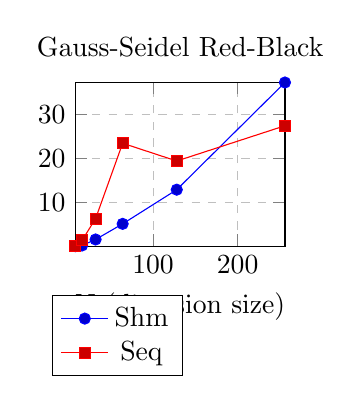
\begin{tikzpicture}
\begin{axis}[
title={Gauss-Seidel Red-Black},
xlabel={N (dimesion size)},
ymajorgrids=true,
xmajorgrids=true,
grid style=dashed,
enlargelimits=false,
scaled y ticks=false,
width=0.35\textwidth, 
legend style={at={(0.2,-0.30)},anchor=north,legend columns=1},
% legend style={legend pos=south east, font=\fontsize{4}{5}\selectfont},
]

\addplot coordinates {
(8       , 0.065786  )
(16      , 0.230133  )
(32      , 1.58636   )
(64      , 5.13336   )
(128     , 12.8914   )
(256     , 37.2239   )
}; \addlegendentry{Shm}

\addplot coordinates {
(8       , 0.120597 )
(16      , 1.37933  )
(32      , 6.32938  )
(64      , 23.4308  )
(128     , 19.3997  )
(256     , 27.4063  )
}; \addlegendentry{Seq}
\end{axis}
\end{tikzpicture}

\pagebreak

Performance of shared version vs distributed (CHAPEL) with number of locales = 2 (gets worse with
higher number of locales - not shown):\\

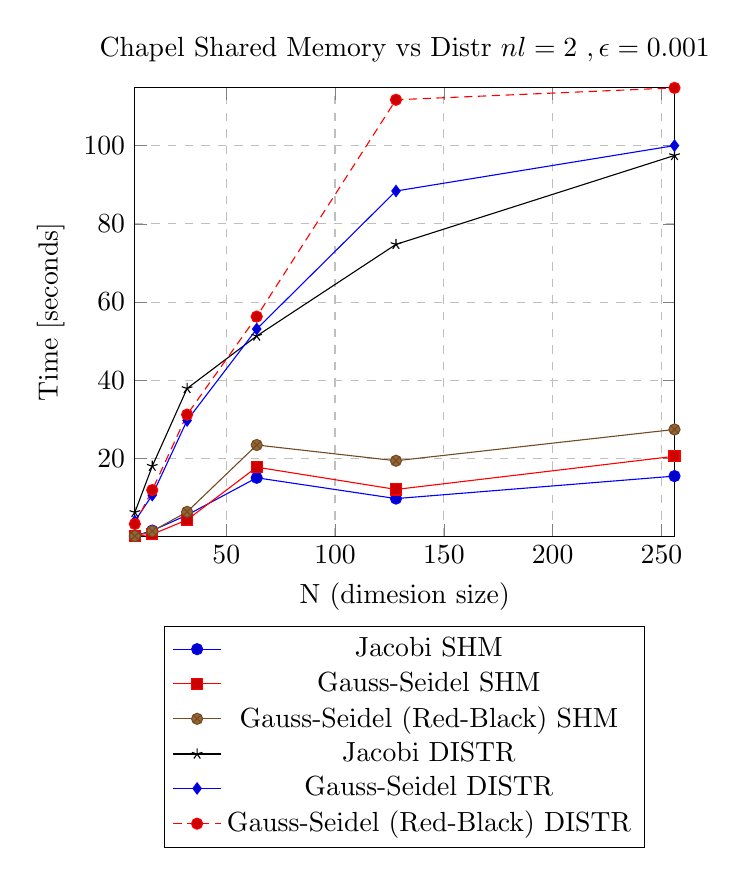
\begin{tikzpicture}
\begin{axis}[
title={Chapel Shared Memory vs Distr  $nl =2\ ,\epsilon = 0.001$},
xlabel={N (dimesion size)},
ylabel={Time [seconds]},
ymajorgrids=true,
xmajorgrids=true,
grid style=dashed,
enlargelimits=false,
scaled y ticks=false,
legend style={at={(0.5,-0.20)},anchor=north,legend columns=1},
]

\addplot coordinates {
(8       , 0.169748  )
(16      , 1.53658   )
(32      , 5.50225   )
(64      , 15.0425   )
(128     , 9.71945   )
(256     , 15.4735   )
}; \addlegendentry{Jacobi SHM}

\addplot coordinates {
(8       , 0.096871   )
(16      , 0.572665   )
(32      , 4.27667    )
(64      , 17.764     )
(128     , 12.0583    )
(256     , 20.5423    )
}; \addlegendentry{Gauss-Seidel SHM}

\addplot coordinates {
(8       , 0.120597 )
(16      , 1.37933  )
(32      , 6.32938  )
(64      , 23.4308  )
(128     , 19.3997  )
(256     , 27.4063  )
}; \addlegendentry{Gauss-Seidel (Red-Black) SHM} 
\addplot coordinates {
(8       , 6.20101   )
(16      , 18.0123   )
(32      , 37.8936   )
(64      , 51.3213   )
(128     , 74.7584   )
(256     , 97.5113   )
}; \addlegendentry{Jacobi DISTR}

\addplot coordinates {
(8       , 3.94065 )
(16      , 10.6155 )
(32      , 29.7121 )
(64      , 53.1043 )
(128     , 88.4176   )
(256     , 100.038   )
}; \addlegendentry{Gauss-Seidel DISTR} 

\addplot coordinates {
(8       , 3.22486 )
(16      , 11.8998 )
(32      , 31.2054 )
(64      , 56.2863 )
(128     , 111.76  )
(256     , 114.807 )
}; \addlegendentry{Gauss-Seidel (Red-Black) DISTR}

\end{axis}
\end{tikzpicture}

\end{document}
